\documentclass[11pt,a4paper]{article}
\usepackage[T1]{fontenc}
\usepackage[utf8]{inputenc}
\usepackage[french]{babel}
\usepackage{lmodern}
\usepackage{graphicx}
\usepackage{geometry}
\geometry{margin=2.1cm}
\pagestyle{empty}
\setlength{\parindent}{0pt}
\setlength{\parskip}{5pt}

\begin{document}
\begin{center}
{\LARGE\bfseries Deux cuves : reprise de l'exercice sous MATLAB}\\[4pt]
{\large Simulink, Stateflow et interface de supervision}\\[8pt]
Birane Diaw --- 4GESI-G1, EMSI Rabat\\
Octobre 2026
\end{center}

\section*{Objet}
Ce travail reprend l'exercice des deux cuves proposé par B. Najimi dans un environnement de simulation MATLAB. Il représente la séquence de commande d'une CPU 1516-3 PN/DP, les entrées et sorties déportées ET200M, le procédé hydraulique et les échanges cycliques d'un maître PROFIBUS DP. L'objectif est de voir et de vérifier le comportement de l'automatisme, notamment lors d'un défaut de liaison.

\section*{Réalisation}
Le modèle Simulink contient deux automates Stateflow. \texttt{Sequence} commande le remplissage de la cuve A par VA-01 pendant 10 s, puis par VA-02 pendant 5 s, l'agitation pendant 15 s, et le transfert vers B par VA-03 et la pompe. \texttt{DP\_Control} représente l'attente, le paramétrage, la configuration, l'échange cyclique et le défaut de communication. Le procédé calcule les volumes et les niveaux des deux cuves à pas de 10 ms. Une IHM MATLAB permet de démarrer, suivre les niveaux et les états, injecter des défauts et exporter les traces.

\begin{figure}[h]
\centering
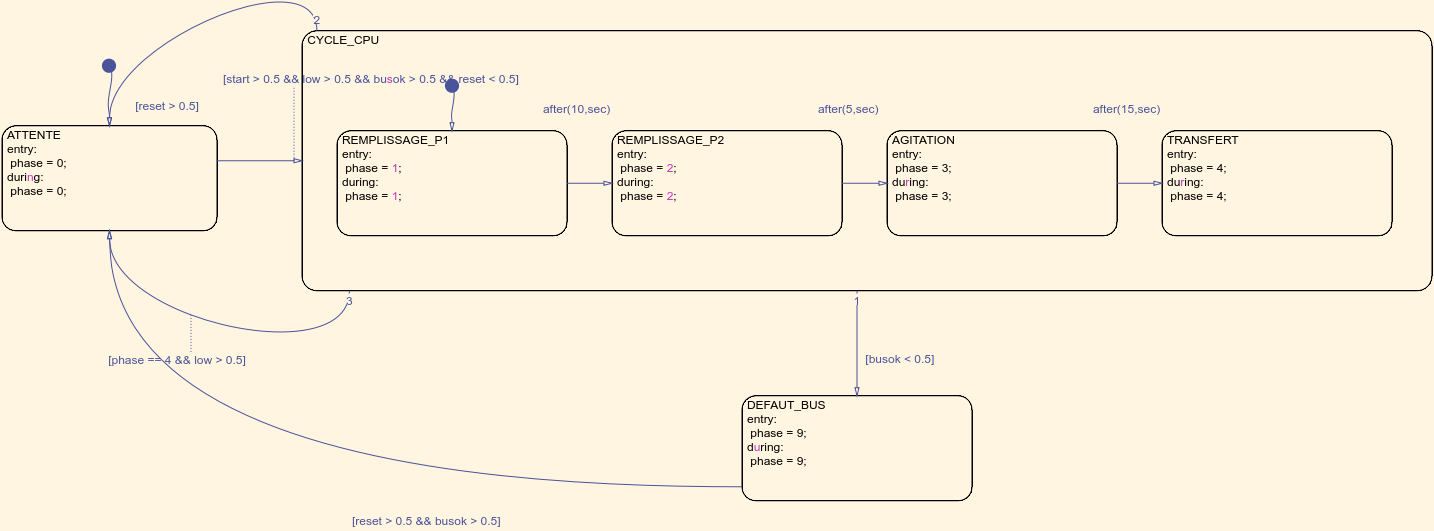
\includegraphics[width=0.94\linewidth]{images/chart_sequence.png}
\caption{Automate de la séquence dans Stateflow (capture du modèle).}
\end{figure}

\clearpage
\section*{Essais et résultats}
Sept scénarios ont été exécutés sous MATLAB R2024a ; les assertions sont toutes satisfaites. Ils couvrent le cycle normal, le démarrage déporté, la cuve B pleine, une perte de liaison, une vanne bloquée, une coupure pendant le remplissage et une remise à zéro pendant le remplissage. Lors d'une coupure du bus, l'échange cesse, les sorties passent à l'état sûr et le défaut apparaît dans l'IHM.

\begin{figure}[h]
\centering
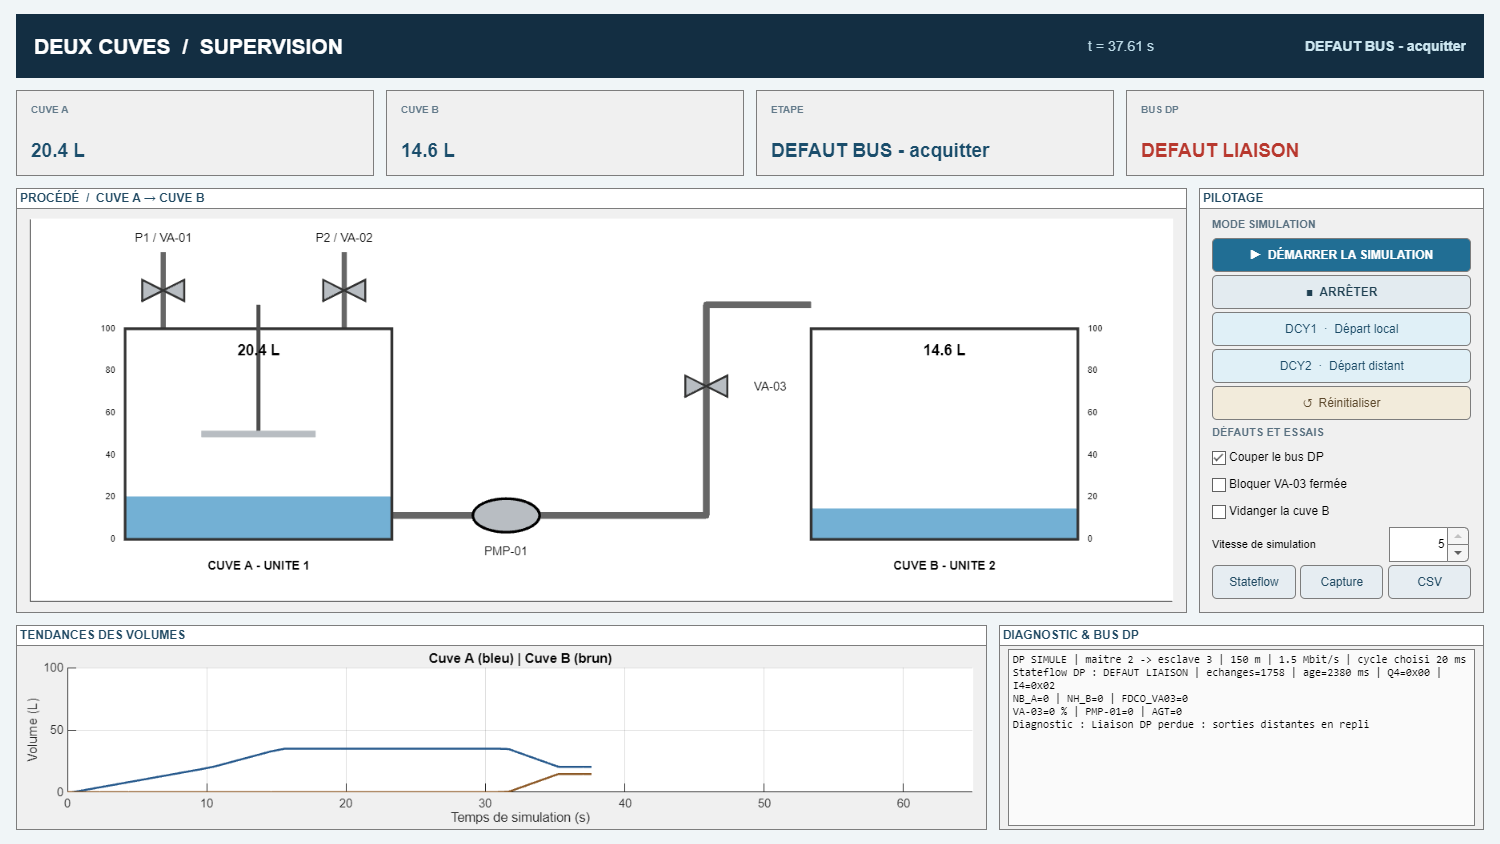
\includegraphics[width=0.96\linewidth]{images/ihm_defaut_bus.png}
\caption{IHM pendant l'essai de perte de liaison (capture de la simulation).}
\end{figure}

\section*{Portée et reproduction}
La liaison DP est une émulation fonctionnelle : aucun télégramme PROFIBUS n'est envoyé sur un bus RS-485 et aucun automate physique n'est connecté. Les temps du cycle émulé (20 ms) et du watchdog (100 ms) sont des choix de démonstration. Pour reproduire les essais, ouvrir le dossier du projet dans MATLAB, exécuter \texttt{demarrer\_projet}, puis \texttt{addpath('matlab'); validate\_cuves}. Les sources, le modèle \texttt{.slx}, les traces et l'IHM sont fournis dans le même dépôt.

\end{document}
